%% Capi: En los capítulos 3 y 4 puedes coger texto del documento que tenemos hecho con Giuseppe, y del proyecto tuyo de tesis.
\chapter{Problem Formulation}
\label{ch:ProblemFormulation}
\lettrine[lraise=-0.1, lines=2, loversize=0.2]{A}{s} mentioned in Chapter \ref{ch:Introduction}, the context around which this cognitive task planner is being developed is the inspection and maintenance of electrical networks. Although one of the objectives is to build a task planner whose characteristics allow its easy reuse and adaptation for other applications, it is relevant to state the problem for which it is being originally prepared. 

As already mentioned, the AERIAL-CORE project aims to develop different technologies for the use of multi-\gls{UAV} system in inspection and maintenance tasks in high-voltage electrical installations. In particular, one of the technologies proposed is the use of \glspl{ACW}, i.e. small teams of cooperative \glspl{UAV} to safely support maintenance workers while working at height on power lines. These systems would have to interact with humans (see Figure \ref{fig:aerial_co_worker}) to inspect certain parts that are indicated to them, monitor worker safety during operation and deliver tools or other light equipment, in order to make the work more efficient and safer. In addition, to have a greater impact, the system would need to operate over extended periods of time, being able to autonomously deal with certain faults or recharges.

\begin{figure}[htbp]
    \centering
    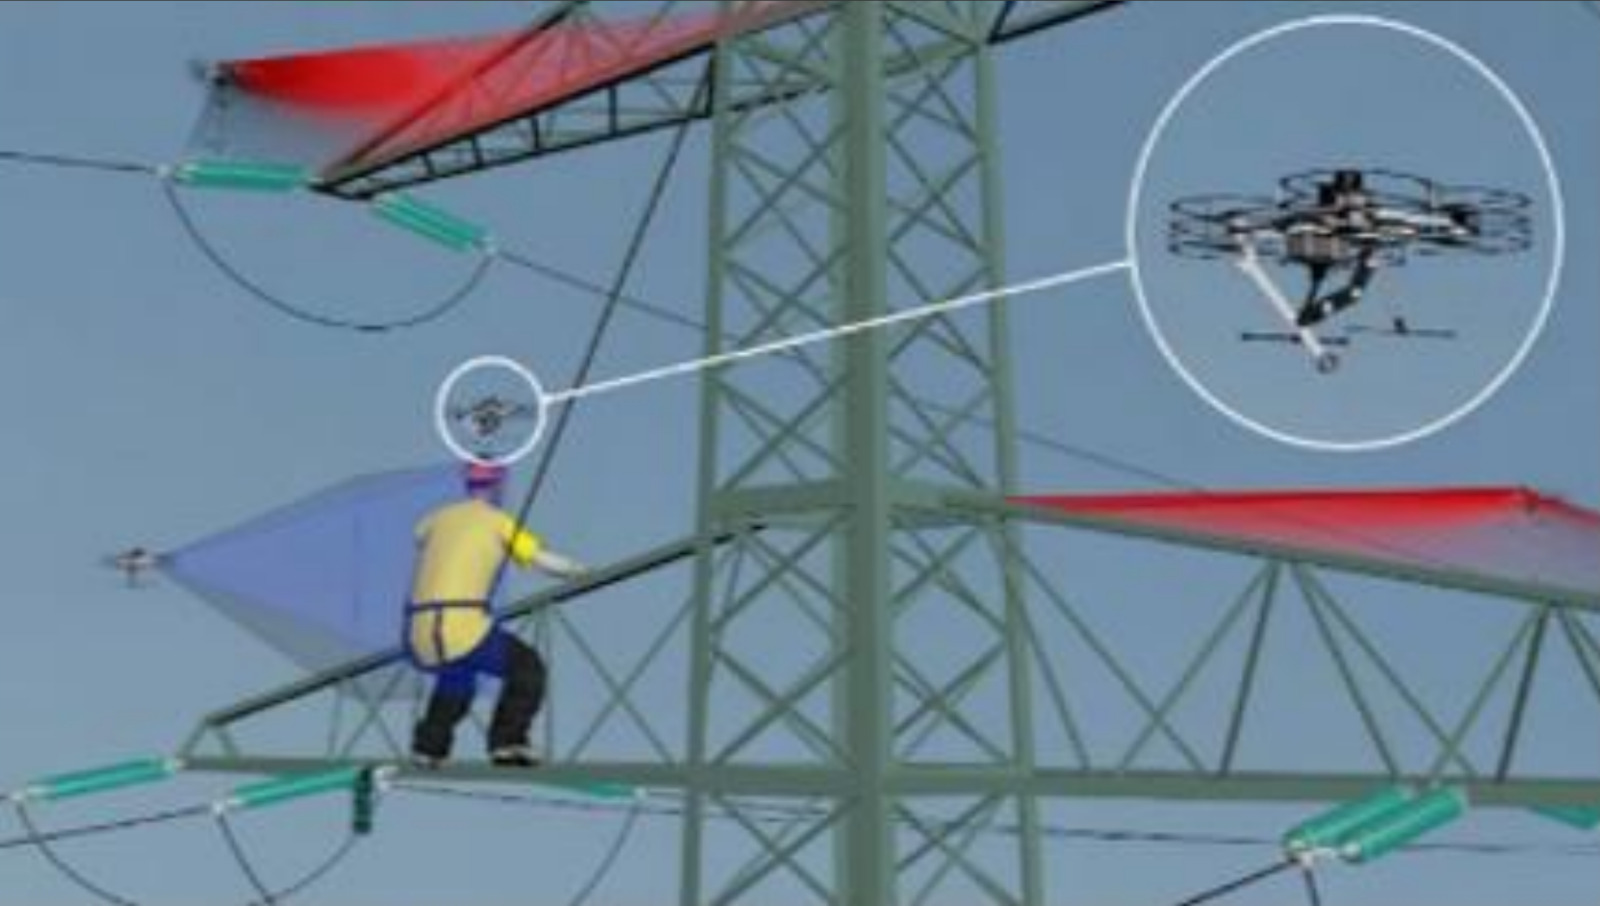
\includegraphics[width=.75\linewidth]
    {ProblemFormulation/figures/aerial_co_worker.jpeg}
    \caption{Multi-\gls{UAV} team supporting an operator. Source: \href{https://aerial-core.eu/}{Aerial-Core website}}
    \label{fig:aerial_co_worker}
\end{figure}

Three types of \glspl{ACW} are referred, each intended to provide different functionality: \textit{Inspection-ACW}, \textit{Safety-ACW}, and \textit{Physical-ACW}. The use case scenarios can be summarized as follows: 

\begin{itemize}
    \item \textit{Inspection}, where a fleet of \glspl{ACW} (i.e., \textit{Inspection-ACWs}) carries out a detailed investigation of power equipment autonomously, helping the human workers to acquire views of the power tower that are not easily accessible (see Figure \ref{fig:inspection_task});
    \item \textit{Safety}, where a formation of \glspl{ACW} (i.e., \textit{Safety-ACWs}) provides the supervising team with a view of the humans working on the power tower in order to monitor their status and to ensure their safety (see Figure \ref{fig:monitor_task});
    \item \textit{Physical}, where an \gls{ACW} (i.e., \textit{Physical-ACW}) physically interacts with the human worker and provides physical assistance to it, i.e., while in contact with the human it flies stably, reliably, and accomplishes the required physical task (e.g., handover of a tool) without becoming harmful for the human worker (see Figure \ref{fig:deliver_task}).
\end{itemize} 

Even if there is a specific type of \gls{ACW} for each of the tasks (inspection, monitoring and tool delivery), this does not mean that a \gls{UAV} can at any given time undertake a task for which it is not the best. It will therefore be the planner's task to take into account which \glspl{ACW} are best suited for each task, which are not but could perform it without problem, and which do not have the capacity to perform it at all. As a consequence, the number of ways in which the mission planning can be carried out multiplies, thus considerably increasing the difficulty of the problem that the task planner has to solve.

This mission planning problem with multiple \glspl{UAV} with battery constraints can be posed as an optimization problem, the solution of which indicates the most efficient way to allocate the different tasks and plan recharges. To react to possible failures, one of the most widespread options is to come up with dynamic methods that can replan in real time as certain events occur. Although there are many variants, most formulations for missions where multiple vehicles visit multiple locations to inspect or make deliveries give rise to NP-hard optimization problems and, therefore, the most widespread approach is to solve them using heuristic algorithms.

Planning methods based on uncertainties are appropriate for adding cognitive capabilities to a system that has to interact with humans in dynamic environments, as they allow optimizing plans by predicting the most likely intentions of humans and the outcomes of future actions. The main problem is their computational complexity, as the plan search space would grow exponentially with the number of \glspl{UAV} and with the future time horizon over which planning is to take place.

It is in this context and with these ideas in mind, the cognitive task planner in this thesis was developed. As this cognitive planner is a module part of a bigger software architecture to tackle the whole problem, the complete picture of that architecture is briefly introduced. Mainy, which information exchanges exist between the upper and lower layers of the software architecture, the interfaces by which this information travels, and the interactions between layers to activate low-level controllers. In the following section this information is presented by individually explaining the different tasks contemplated in the project. 

Additionally, a review will be made of other important considerations that the planner has to take into account, such as battery recharges, connection losses and task rescheduling; analyzing the different situations in which each of them can occur and their different causes. 

\section{Description of tasks}
\label{sec:DescriptionOfTasks}
As mentioned above, three different types of tasks are envisaged in the project. These tasks are requested at any time by human workers through gestures. There will be a higher level software layer that processes the information contained in the gestures so that the planner receives an asynchronous communication from the upper layer containing the specifications of a new task. At this point, it is the planner's job to process the new information together with the information it already had in order to elaborate and implement a new plan. The same planner is also in charge of calling the low-level controllers when necessary and ensuring the safety of the \glspl{UAV} and the fulfillment of the mission. Each task is explained in detail in the following sections.

\subsection{Inspection tasks}
\label{subsec:InspectionTasks}
This task can be performed by all three types of \glspl{ACW}. It is the second highest priority task, with the tool delivery task being the only one that exceeds it. It consists of carrying out a detailed inspection of the specified areas of the power equipment. The layer immediately above the task planner is responsible for passing it a list of \glspl{WP} that define the inspection task, and the planner is responsible for deciding how many \glspl{ACW} it recruits to execute the task and which of the available \glspl{ACW} it assigns it to. Dividing the total \gls{WP} list to be inspected into subsets and assigning each one to one of the \glspl{ACW} selected for the task is the job of a low-level controller. Therefore, once the planning is executed, the tasks of this type are transmitted to the lower level layers with the total list of \glspl{WP} to be re-inspected and a list with the \glspl{ID} of the selected \gls{UAV}.

All the aforementioned communications will be carried out asynchronously, as the creation of the task by the workers, which triggers the whole sequence of actions, is done in this way.

\begin{figure}[htbp]
    \centering
    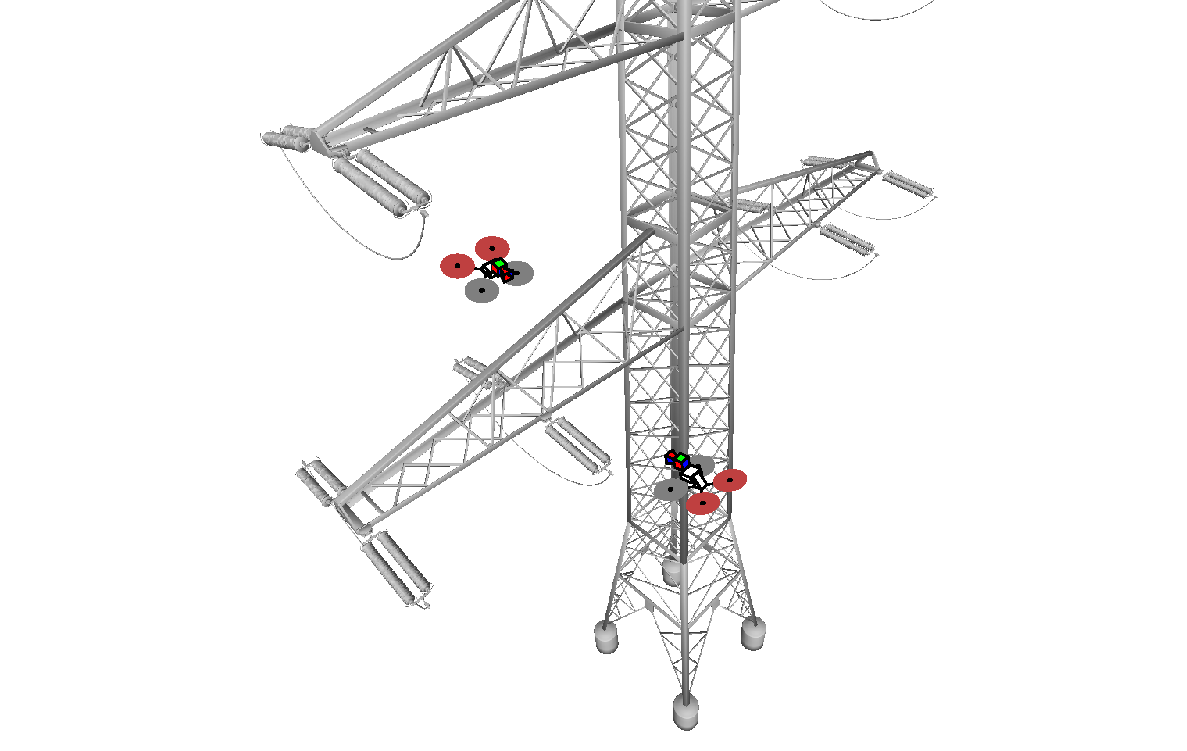
\includegraphics[width=.75\linewidth]
    {ProblemFormulation/figures/inspection_task.pdf}
    \caption{\textit{Inspection-ACW} carrying out an inspection task}
    \label{fig:inspection_task}
\end{figure}

\subsection{Monitoring tasks}
\label{subsec:MonitoringTasks}
This task can also be executed by all three types of \glspl{ACW}. It is the lowest priority task. Monitor worker's safety consists of providing the supervisory team with a view of the people working in the power tower to monitor their status and ensure their safety. The layer immediately above the task planner communicates this time the \gls{ID} of the worker to be monitored, the number of \glspl{UAV} desired and the distance they should keep from the worker. It is the task planner's responsibility to decide once again which of the available \glspl{ACW} to assign to this task and the formation they should maintain during the flight. Once the planning has been carried out, the tasks of this type are passed on to the lower level layers with both the original information and the information resulting from the planning.

The aforementioned communications will also be carried out asynchronously for the same reason. 

\begin{figure}[htbp]
    \centering
    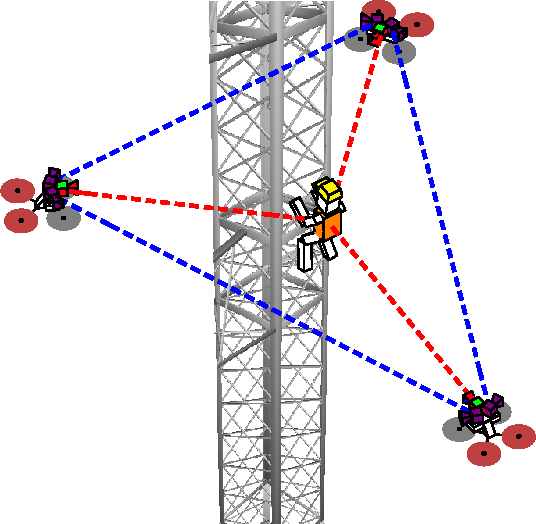
\includegraphics[width=0.5\linewidth]
    {ProblemFormulation/figures/monitor_task.pdf}
    \caption{\textit{Safety-ACW} carrying out a monitoring task}
    \label{fig:monitor_task}
\end{figure}

\subsection{Tool delivery tasks}
\label{subsec:ToolDeliveryTasks}
This task can be performed only by \textit{Physical-ACW} \glspl{UAV}, as special hardware is required to perform the physical interaction with the low-weight objects and the human. This is the highest priority task. Delivering a tool consists of picking up a tool and transporting it to the worker, with whom a physical interaction will take place through which the delivery of the tool will take place. Low-level controllers will have to be especially precise and careful not to hurt the worker. This time, the layer immediately above the task planner communicates the \gls{ID} of the worker to whom the tool is to be delivered and the \gls{ID} of the requested tool. Again, the task planner's mission is to decide to which of the available \glspl{ACW} assign this task. Once the planning is carried out, tasks of this type are passed on to the lower level layers with the same information as originally.

The aforementioned communications, once again, will be carried out asynchronously. 


\begin{figure}[htbp]
    \centering
    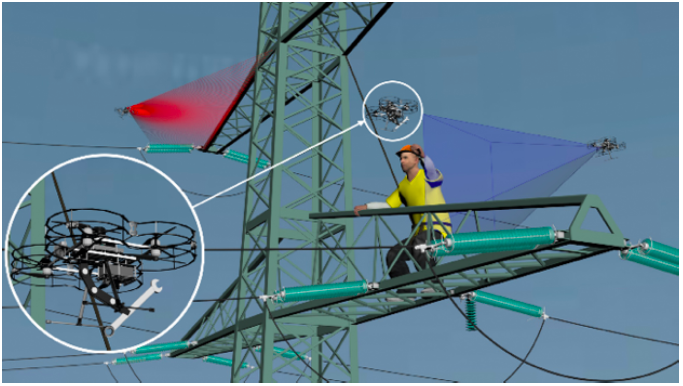
\includegraphics[width=0.7\linewidth]
    {ProblemFormulation/figures/deliver_task.png}
    \caption{\textit{Physical-ACW} carrying out a tool delivery task}
    \label{fig:deliver_task}
\end{figure}

\section{Battery recharges}
\label{sec:BatteryRecharges}
Given the current autonomy problem with \gls{UAV} technology, eventually each of the \glspl{ACW} involved in the mission will run out of battery power. The moment when the battery of each one will run out can be estimated from the mission planning itself, so the planner can take this into account when distributing the tasks so that the \gls{ACW} itself anticipates this event. Recharging does not necessarily have to take place when the \gls{UAV} is about to run out of battery, nor does it have to take place until the battery reaches its maximum, but both will be parameters to be taken into account during the mission planning and optimization process.

Besides, it is possible that the calculations may fail for some reason, and the battery may run out sooner than expected. It will therefore be necessary to periodically read the battery status and perform emergency recharging and replanning if necessary, reacting to unexpected faiulres. One possible scenario is that the aerial robot runs out of battery during a loss of connection. Since the planner is centralised at a ground station, there should also be a battery check and action module on board each aerial vehicle, and an emergency protocol in case this happens.

In the absence of specifications, it is assumed that battery recharging does not occur instantaneously (it is not a battery change), so reaching the desired battery level takes a certain amount of time that should be considered in the plan.

Also, the task planning algorithm has to be able to handle without blocking situations where all \glspl{ACW} are simultaneously without sufficient battery power and therefore there is no \gls{UAV} with which to execute a task immediately.

\section{Connection losses}
\label{sec:ConnectionLosses}
Another important consideration is the possible loss of connection between the centralised planner, where most of the cognitive capacity is concentrated, and one of the \glspl{ACW}. Since a loss of connection is an unforeseen event, it is most likely that the planner will recalculate the optimal task allocation once the \gls{UAV} fleet is updated, so that the tasks previously assigned to the disconnected \gls{ACW} will be executed on another one. This is a potentially dangerous situation because the disconnected \gls{UAV} could act autonomously according to its last plan and cause an accident with the rest of the agents that are still online.

It is therefore important: (i) to implement a system to detect disconnections from both sides of the communication, and (ii) to establish a common action protocol so that both modules know how the other is going to act, thus ensuring the integrity of all vehicles and the safety of the workers.

\section{Task replanning situations} % Unforeseen events
\label{sec:TaskReplanningSituations}
Once the mission is underway, any unforeseen event has the potential to completely change which the optimal plan is. Therefore, even if there is a possibility that the event will not affect the mission at all, it will always be necessary to execute a mission replanning in case of an unforeseen event.

The following is a list of the unforeseen events that have been contemplated in this work:

\begin{itemize}
    \item Arrival of a new task.
    \item Modification of a task's parameters.
    \item Connection of a new \gls{ACW}.
    \item Disconnection of an \gls{ACW}.
    \item Unplanned insufficient battery in one of the \glspl{ACW}.
    \item Battery drain faster than expected and therefore will not be enough for the current plan.
    \item An \gls{ACW} finishes recharging ahead of schedule.
    \item A task is successfully completed.
    \item A task is completed unsuccessfully.
\end{itemize}

Note that some of the events considered are not really unexpected. Successful completion of a task is what is desired, for example, so it should not imply a change of plans. However, this event is included in the list because it is a good moment to check if there is a better plan and to modify the current one if necessary. As the planner is pursuing the optimal plan, the result of the replanning will keep the previous plan unchanged if it is still optimal.